%!TEX root = ../thesis_a4.tex

\chapter{Background}
\label{chap:background}

\section{Introduction}

In this chapter we provide the relevant music and scientific background for the work presented in this dissertation. We start with a brief discussion on the terminology used in this thesis (\secref{sec:background_terminology}). Subsequently, we provide an overview of the selected music concepts relevant to better understand our work (\secref{sec:music_background}). We then present a review of the literature related with the topics addressed in this thesis. We first present relevant work done in computational analysis of \gls{iam} (SEction XX), which includes approaches for tonic identification, automatic \gls{raga} recognition and melodic pattern processing. Then, we present work done for other music traditions within \gls{mir} on topics covering melodic pattern processing and key recognition (\secref{sec:background_relevant_work_other_music}). Finally, we provide an overview of the select scientific concepts in information retrieval, time-series analysis, complex networks and statistics (\secref{sec:background_scientific_background}). We conclude this chapter by providing a summary of the literature review, wherein we highlight the shortcomings of the existing approaches, and identify some possible venues for scientific contribution (\secref{sec:background_summary}). 

\section{Terminology}
\label{sec:background_terminology}

In this section we provide working definition of the selected terms we have used throughout the thesis. Since the thesis focuses on the melodic description of \gls{iam}, it is important to clearly understand the meaning of melody in the context of this thesis. Our aim here is not to formally define melody in an universal sense, which as we see from the literature has been a challenge in itself, with almost every definition falling short of considering some aspect or the other XXXX. It would not be an overstatement to say that there is no agreed definition of melody that suits every context. For a review of interesting definitions of melody we refer to XXXX. Before we present the definition of melody that we consider in this work, it is important to understand the performance or concert setup in \gls{iam}. Since this music tradition is performance-based, even the studio recordings follow the same setup. Performances in \gls{iam} have a clearly defined concept of a lead artist, who plays the central role (also literally positioned in the center of the stage) and all other instruments are considered the accompaniments. In this context, mergin relevant parts of the definitions given by~\cite{paiva2006melody,kim2000analysis,levitin2002memory} covers to a large extent the scope of melody in \gls{iam}. Their definitions in the respective order are: \textquote{``\textit{the dominant individual pitched line in a musical ensemble}''} and \textquote{``\textit{an auditory object that emerges from a series of transformations along the six dimensions: pitch, tempo, timbre, loudness, spatial location, and reverberant environment}''}.  The first definition falls short of considering several other dimensions of sound such as timbre and loudness that are important in perception and production of melody, which are taken into account in the second definition. The concept of audio as a mixture of sounds from multiple instruments (`\textit{ensemble}') is missing in the second definition, which the first definition takes into account. The idea of continuity and smoothness of melody is expressed by `\textit{line}' in the former and by `\textit{series of transformations}' in the latter. If we combine these two definitions we can rewrite our working definition as \textquote{``\textit{an auditory object that emerges from a continuous series of transformations along the six dimensions: pitch, tempo, timbre, loudness, spatial location, and reverberant environment, by the dominant individual sound source in a music ensemble}''}. Although, we only consider the pitch dimension of melody in this thesis. Thus, loosely speaking, for all practical purposes within the scope of this thesis, we represent melody by a continuous pitch time-series corresponding to the lead artist in an audio recording, also referred to as predominant pitch in the subsequent chapters. This definition does not explicitly take into account the rare case of two lead artists. Since in a majority of such cases the two lead sound sources are active sequentially in time, our definition encompasses this scenario by considering the active sound source as dominant. \TODO{please make this shit better, these thigns are so confusing and broad}

Now that we have a working definition of melody, we proceed to define the scope of the terms such as melodic patterns, phrases and motifs in this thesis, and disambiguate them with other seemingly synonymous terms such as melodic fragment and segment. Melodic fragment or melodic segment in this thesis refers to a continuous subsequence of the pitch sequence. It does not entail any musical relevance in terms of the boundaries or the length of the subsequence. By a melodic pattern we refer to a repeating melodic fragment, where the scope and the meaning of repetition is based on the perceived melodic similarity. Across repetitions, a melodic fragment can undergo a series of time and pitch transformations allowed within the periphery of melodic framework (\gls{raga} in our case) without altering the identity of the melodic unit. Also, the melodic similarity here refers to the perceived similarity between melodic fragments when heard in isolation, as the local melodic context can influence the perception of similarity. Melodic patterns in this thesis do not entail any particular musical significance in terms them being characteristic of a melodic concept in \gls{iam}. The terms melodic pattens, fragments and segments are more from the perspective of signal or the time-series. Melodic phrases on the other hand are used in the context of music, as being a unit of melody which encapsulate an idea or a musical thought by an artist. Melodic motif is further high-level concept and we use it to refer to a particular type of characteristic patterns, in out thesis of \glspl{raga}, \gls{raga} motifs. 


The word polyphonic in the context of audio recordings signifies that the recordings consists of a mixtue of multiple instruments playing simultaneously.


\section{Music Background}
\label{sec:music_background}

\subsection{Indian Art Music}

\subsection{Melodies in Indian Art Music}

\subsubsection{Tonic in Indian art music}
\label{sec:background_tonic_in_iam}

\subsubsection{Svaras}

\subsubsection{Aroh-Avroh}

\subsubsection{Gamakas and Ornaments}

\subsubsection{Raga in Indian Art Music}

\paragraph{Phase-based and Scale-based ragas}
\paragraph{Allied ragas}

\subsubsection{Characteristic Melodic Phrases}

\subsubsection{Chalan}

\subsubsection{Nyas}
\label{sec:backgroung_nyas_description}

Dey presents various interpretations and perspectives on the concept of ny\={a}s in Hindustani music according to ancient, medieval and modern authors~\cite{Dey2008}. In the context of its current form, the author describes ny\={a}s as that process in a performance of a r\={a}g where an artist pauses on a particular svar\footnote{The seven solf\`{e}ge symbols used in Indian art music are termed as svars. It is analogous to note in western music but conceptually different.}, in order to build and subsequently sustain the format of a r\={a}g, the melodic framework in Indian art music~\cite[p. 70]{Dey2008}\cite{KKG_SS13}. Dey elaborates the concept of ny\={a}s in terms of action, subject, medium, purpose and effect associated with it. Typically, occurrence of a ny\={a}s delimits melodic phrases (motifs), which constitute one of the most important characteristic of a r\={a}g. Analysis of ny\={a}s is thus a crucial step towards melodic analysis of Hindustani music. In particular, automatically detecting occurrences of ny\={a}s (from now on referred as ny\={a}s segments) will aid in computational analyses such as melody segmentation, motif discovery, r\={a}g recognition and music transcription~\cite{GopalJNMR2012, Rao2014}. However, detection of ny\={a}s segments is a challenging computational task, as the prescriptive definition of ny\={a}s is very broad, and there are no fixed set of explicit rules to quantify this concept~\cite[p. 73]{Dey2008}. It is through rigorous practice that a seasoned artist acquires perfection in the usage of ny\={a}s, complying to the r\={a}g grammar and exploring creativity through improvisation at the same time. 

\subsubsection{Recurring Melodic Patterns in IAM}


\section{Relevant Work in Indian Art Music}
\label{sec:background_relevant_work_iam}


\subsection{Tonic Identification}
\label{sec:background_relevant_work_tonic_identification}

In this section we provide a detailed review of the existing methods for tonic identification in audio recordings of \gls{iam}. The main objective of this review is to break down the methodology used across methods into a common set of processing blocks, and subsequently analyze different methods in terms of these blocks. Since in this thesis we also perform an extensive comparative evaluation of a number of these methods (\secref{}), we review the methods in detail. In order to better interpret the output of these methods and to relate them with the processing steps and parameter choices, we provide the necessary implementation details, wherever required.


Identification of tonic pitch of the lead artist in an audio recording is a crucial first step in tonal analysis of \gls{iam} (\secref{sec:background_tonic_in_iam}). Knowing the tonic pitch used in an audio recording enables a meaningful comparison of melodies across different artists and their recordings. In this section we review existing approaches for automatic tonic identification in audio collections of \gls{iam}. 

As mentioned, there have been various efforts to automatically identify the tonic pitch of the lead artist in a performance of Indian art music~\citep{salamon2012multipitch,gulati2012two,bellur2012knowledge,ranjani2011carnatic,Sengupta2005b}. These approaches mainly differ in terms of the musical cues that they utilize to identify the tonic, the amount of input audio data used to perform this task and the type of music material they are devised for (Hindustani or Carnatic, vocal or
instrumental, etc.). Despite the differences, all these approaches can be divided into three main processing blocks, as shown in~\figref{fig:tonic_identification_general_block_diagram}. The only exception to this schema is the approach proposed by~\cite{Sengupta2005b}.

\begin{figure}
	\begin{center}
		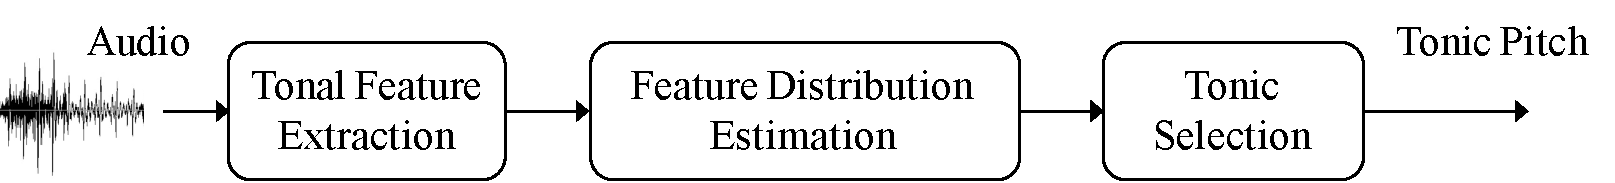
\includegraphics[width=\figSizeNinety]{ch02_background/figures/tonic_identification_block_diagram.pdf}
	\end{center}
	\caption[General block diagram of the processing steps used by tonic identification
	approaches.]{General block diagram of the processing steps used by tonic identification
		approaches.}
	\label{fig:tonic_identification_general_block_diagram}
\end{figure}


In all the aforementioned approaches, the three main processing blocks are the following: feature extraction, feature distribution estimation and tonic selection. Since the task of tonic identification involves an analysis of the tonal content of the audio signal, the features extracted in the first block are always pitch related. In the second block, an estimate of the distribution of these features is obtained using either Parzen window based density estimation or by constructing a histogram. The feature distribution is then used in the third block to identify the tonic. The peaks of the distribution correspond to the most salient pitch values used in the performance (usually the \glspl{svara} of the \gls{raga}), one of which corresponds to the tonic pitch. As the most salient peak in the distribution is not guaranteed to be the tonic, various techniques are applied to select the peak that corresponds to the tonic.

{\renewcommand{\arraystretch}{1.5}
	\begin{sidewaystable} 
		\begin{centering}
			\begin{tabular}{ c c c c }
				\tabletop			
				Method 	&	Features	&	Feature Distribution	&	Tonic Selection \\
				\tablemid			
				\acrshort{tonicid_sengupta} \citep{Sengupta2005b}	&	Pitch \citep{AKDatta_1996} & N/A & Error minimization\\
				
				\acrshort{tonicid_ranjani_1}/\acrshort{tonicid_ranjani_2} \citep{ranjani2011carnatic}	&	Pitch \citep{BoersmaPaul2001} & Parzen-window-based \acrshort{pde}  & GMM fitting\\
				
				\acrshort{tonicid_justin} \citep{salamon2012multipitch} & Multi-pitch salience \citep{Salamon2011} & Multi-pitch histogram & Decision tree\\
				
				\acrshort{tonicid_sankalp} \citep{gulati2012two}	& Multi-pitch salience  \citep{Salamon2011} & Multi-pitch histogram & Decision tree\\
				
				&	Predominant melody \citep{Salamon2012} & Pitch histogram & Decision tree\\
				
				\acrshort{tonicid_ashwin_1} \citep{bellur2012knowledge}	&	Pitch \citep{DeCheveigne2002}	&  \acrshort{gd} histogram & Highest peak\\
				
				\acrshort{tonicid_ashwin_2} \citep{bellur2012knowledge}	&	Pitch \citep{DeCheveigne2002}	& 	GD histogram	&
				Template matching\\
				
				\acrshort{tonicid_ashwin_2} \citep{bellur2012knowledge}	&	Pitch \citep{DeCheveigne2002}	& 	GD histogram
				& Highest peak\\
				
				\acrshort{tonicid_chordia}	& 	& 	& \\			
				
				\tablebot			
			\end{tabular}
			
			\caption[Summary of existing tonic identification approaches.]{Summary of existing tonic identification approaches.}
			\label{tab:pre_processing_tonic_identification_summary_methods}
			\par \end{centering}	
	\end{sidewaystable}
	
	
In \tabref{tab:pre_processing_tonic_identification_summary_methods} we provide a summary of the existing methods for tonic identification. The common processing blocks and the main differences between them become evident from this table. A detailed review of these methods in terms of the three processing stages as shown in \figref{fig:tonic_identification_general_block_diagram} is done in~\cite{Gulati2014Tonic}. For a more detailed description of these methods we refer to their respective publications listed in Table \tabref{tab:pre_processing_tonic_identification_summary_methods}. 


\subsubsection{Tonal Feature Extraction}
\label{Feature Extraction}

In the tonal feature extraction block (\figref{fig:tonic_identification_general_block_diagram}), the algorithms extract pitch-related
features from the audio signal for further processing. With the exception of \cite{SalamonSankalp2012,SGulatiIstanbul2012}, all approaches use a single feature, the predominant pitch in the audio. Note that whilst pitch and fundamental frequency ($f_0$) are not the same (the former being a perceptual phenomenon and the latter a physical quantity), for the purpose of tonic identification the $f_0$ is considered a reliable representation of pitch. Unlike these approaches, Salamon \cite{SalamonSankalp2012} uses a multi-pitch salience feature in order to exploit the tonal information provided by the drone instrument. Finally, Gulati \cite{SGulatiIstanbul2012} uses both the multi-pitch salience feature and the predominant melody. 

We now provide an overview of the algorithms used by the different approaches mentioned above for extracting $f_0$ and multi-pitch salience from audio recordings. \cite{ranjani2011carnatic} use the Praat software\footnote{Version 5.3.} \cite{BoersmaPaul2001} to obtain the pitch contours. The software implements the algorithm by~\cite{boersma1993accurate}, which is primarily proposed for speech signals and has also been used for monophonic music recordings in the past. \cite{Ashwin_Istanbul2012} uses an \gls{amdf} based pitch estimation algorithm, YIN, proposed by~\cite{DeCheveigne2002}. YIN is mainly developed for speech signals. As~\cite{DeCheveigne2002} make a remark,  the algorithm is informally tested on music and yet to be evaluated on polyphonic music. However, YIN has been used in a number of studies in \gls{mir} for pitch estimation from polyphonic music signals REF. \cite{Sengupta2005b} use a method based on \gls{psa} proposed by~\cite{AKDatta_1996} for extracting the $f_0$. Subsequently, a steady state detection is applied to the pitch contours in order to consider only the steady note regions for the analysis. Only segments of the pitch contour with a steady-state duration of at least 60 ms are used. It should be noted that this study was carried out using solo vocal performances (monophonic audio), which were carefully recorded in a studio without any kind of accompaniment present in the audio.

One of the possible caveats of the aforementioned pitch (strictly speaking, $f_0$) estimation methods is that they are all designed for monophonic signals containing a single sound source. This means that the number of estimation errors could increase as we add more instruments into the mixture. While due to the heterophonic nature of \gls{iam} and the prominent lead voice monophonic pitch trackers often manage to detect the $f_0$ of the lead artist even in the presence of accompaniment instruments. One way of overcoming this problem is by using a predominant pitch estimation algorithm. \cite{gulati2012two} use the method proposed by~\cite{Salamon2012} for estimating the pitch sequence of the predominant melody from the audio signal. \cite{gulati2012two} exploit the pitch information of the melody in the second stage of their approach to identify the specific octave of the tonic pitch (the tonic pitch-class is identified during the first stage of the algorithm).

As noted earlier, some recently proposed methods for tonic identification~\citep{salamon2012multipitch,gulati2012two} use a multi-pitch approach. Instead of extracting the predominant melodic component from the audio signal, the methods compute a multi-pitch time-frequency representation of pitch salience over time~\citep{Salamon2011}. The motivation for using multi-pitch analysis is twofold: first, as noted earlier, the music material under investigation is non-monophonic (includes many instruments playing simultaneously). Second, the tonic is continuously reinforced by the drone instrument, and this important cue can not be exploited by only extracting a single pitch value for each frame of the audio recording. To illustrate this point, in~\figref{fig:2HarmonicSeries} we display the spectrogram of a short audio excerpt of Hindustani music. Two types of harmonic series are clearly visible in the plot: the first consists of nearly straight lines and corresponds to the drone instrument (playing Sa and Pa). The second harmonic series (which start approximately at time 1 s) corresponds to the voice of the lead performer. Since the drone instrument is constantly present in the signal, a histogram of the peaks of the salience function will have prominent peaks at the pitches of the drone instrument, and this is exploited by \cite{SalamonSankalp2012,SGulatiIstanbul2012} for identifying the tonic. The main difference between the two approaches is that whilst~\citep{salamon2012multipitch} directly identifies the tonic pitch from the histogram, \cite{gulati2012two} divides the task into two stages: first the tonic pitch-class is identified using an extension of \cite{salamon2012multipitch}, and then the correct tonic octave is identified using the predominant melody information (see~\cite{Gulati2014Tonic} for further details).

\begin{figure}
	\begin{center}
		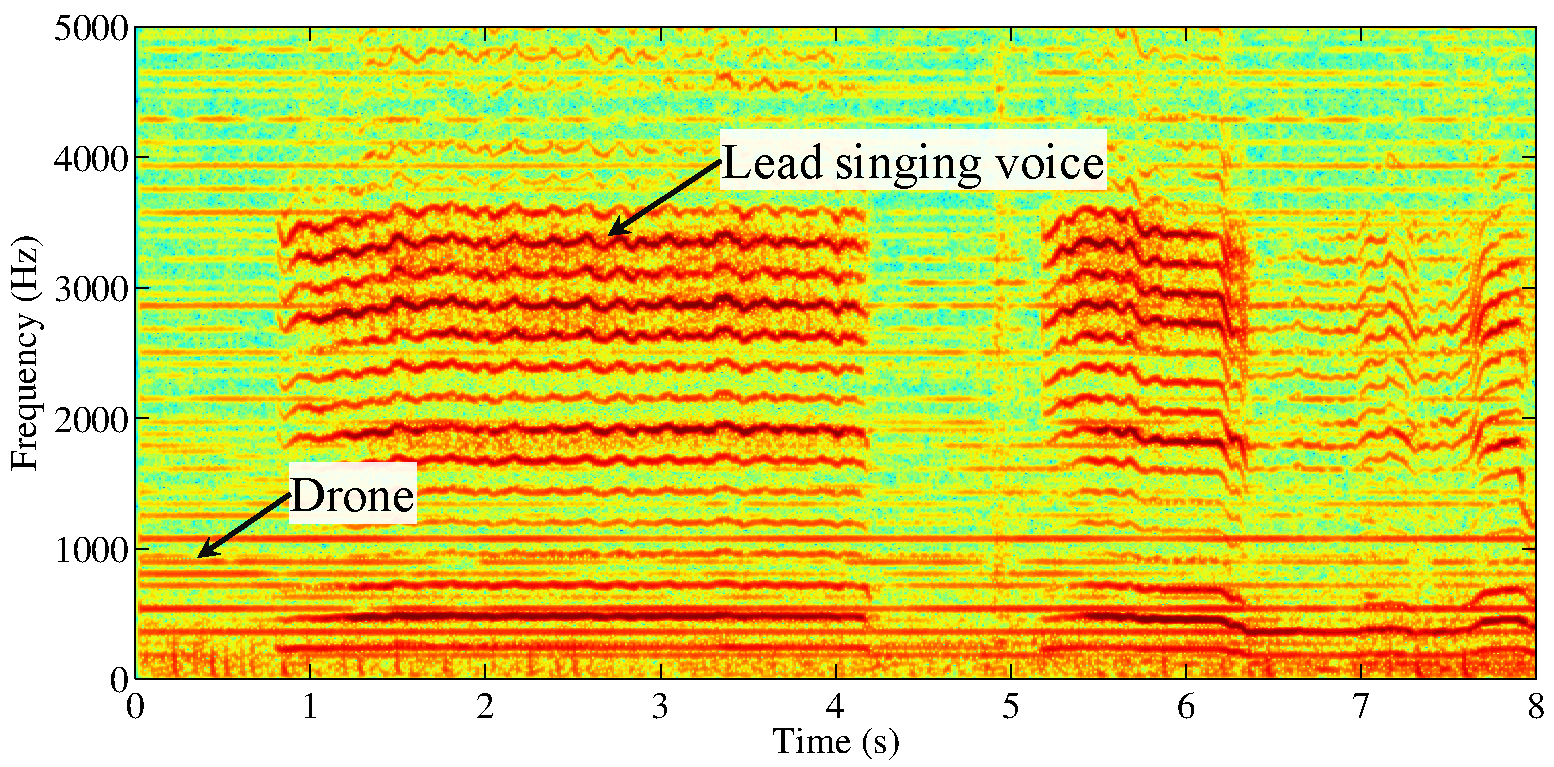
\includegraphics[width=\figSizeNinety]{ch02_background/figures/2HarmonicSeries.pdf}
	\end{center}
	\caption{Spectrogram of an excerpt of Hindustani music with two clearly visible types of harmonic series, one belonging to the drone and the other to the lead voice.}
	\label{fig:2HarmonicSeries}
\end{figure}


\subsubsection{Feature Distribution Estimation}
\label{sec:background_tonic_feature_distribution_estimation}

The tonal features extracted by the different tonic identification approaches are subsequently analyzed in a cumulative manner (cf.~block two in Figure \ref{fig:tonic_identification_general_block_diagram}). The pitch values from all analysis frames (whether a single value is computed per frame or multiple values) are aggregated into a pitch distribution function, which reflects the (possibly weighted) rate of occurrence of different pitch values in the entire audio excerpt. The peaks of the pitch distribution function represent the most frequent (or salient if weighting is used) pitches in the recording, one of which will be the tonic. The only exception is the approach proposed by~\cite{Sengupta2005b}, which instead of analyzing the distribution of the features, computes an aggregate error function in order to select the tonic. The methods used by the different tonic identification approaches for estimating the pitch distribution function are described below.

In \cite{salamon2012multipitch,gulati2012two}, the pitch values of the peaks of the salience function in every frame are aggregated into a histogram. The top 10 peaks in every frame are used, in this way ensuring that in addition to the lead instrument/voice, the pitch content of other accompanying instruments is also captured, most importantly the notes played by the drone instrument. The frequency range considered for selecting the peaks of the salience function for constructing the histogram is restricted to 100-370 Hz (note that the typical frequency range for the tonic 100-260 Hz). The reason for computing the histogram beyond 260 Hz even though the tonic
rarely goes above this frequency is that in some cases the aforementioned methods can exploit the presence of a peak corresponding to the fifth/fourth (Pa/Ma) above the tonic in order identify the tonic pitch.

Since in many cases the lead voice/instrument is considerably louder than the drone sound, the weights of the salience peaks are ignored when computing the histogram, meaning only the rate of occurrence is taken into account. As noted earlier, the result is that the pitches produced by the drone instrument (the tonic and Pa, Ma or Nī) manifest in the form of high peaks in the histogram, since the drone sounds continually in the recording. The resulting pitch distribution thus depends heavily on the notes of the drone instrument. This would not be the case if we only considered the predominant melody for computing the histogram, in which case the pitch distribution would depend on the chosen \gls{raga}, thus increasing the complexity of identifying the tonic.

In Figure \ref{fig:PitchHist} we display two pitch histograms, computed using (a) the pitch of the predominant melody and (b) the peaks of a multi-pitch salience function. Both histograms are computed from the same three-minute audio excerpt. We see that in the histogram computed using the predominant melody (a), the prominent peaks correspond to svars Sa, Ga and Re (the prominent svars of the \textit{Sindh Bhairavī} rāg), whereas in the multi-pitch histogram (b), the top three peaks correspond to Sa (in two octaves) and Pa, which are the prominent svars produced by the drone instrument. 

\begin{figure}
	\centerline{{
			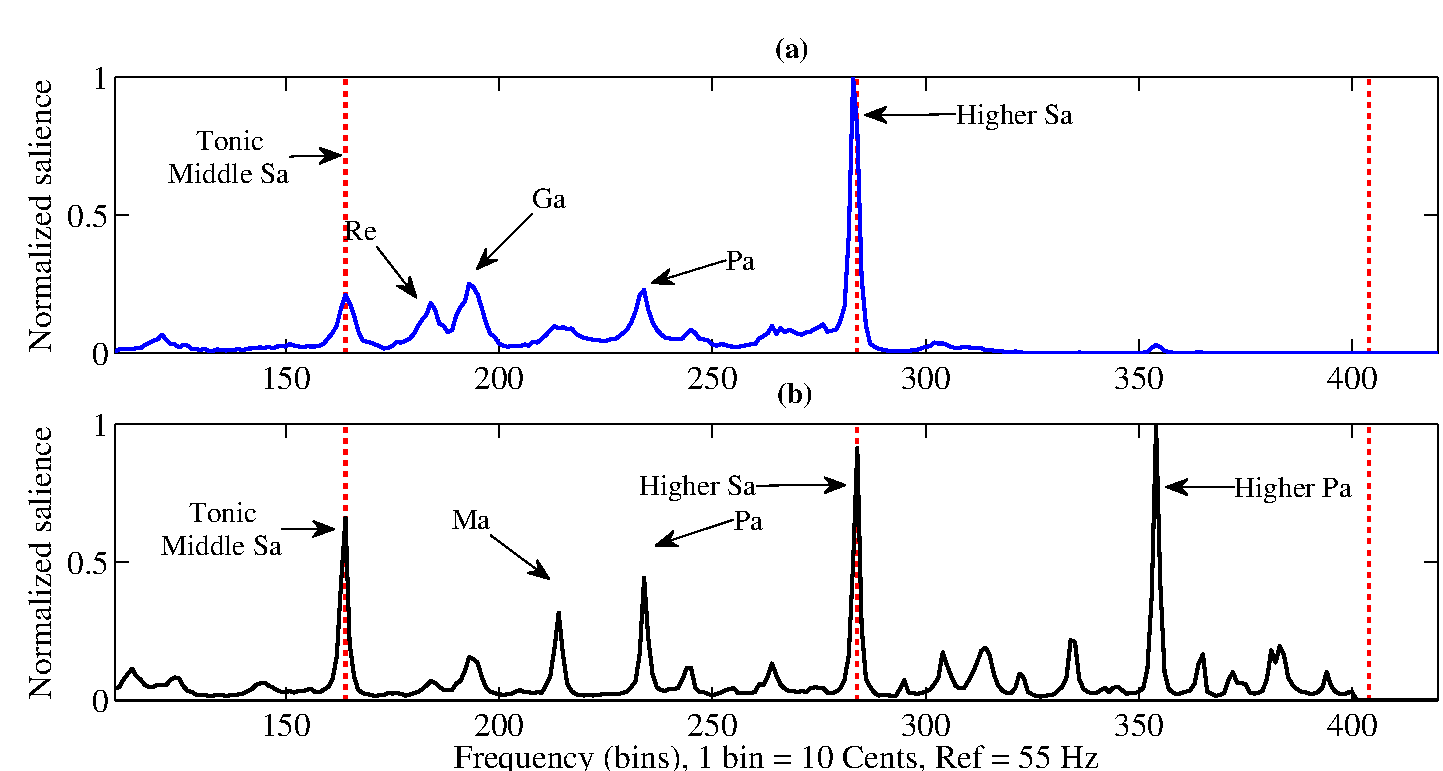
\includegraphics[scale=0.6]{fig/distributions/Histogram_Melody_Multipitch.pdf}}}
	\caption[Comparison of the histograms constructed using different
	methods]{Pitch histograms for the same excerpt constructed using (a)
		predominant melody (in blue) and (b) peaks of a multi-pitch salience function (in black). The tonic
		pitch-class locations are indicated with red dotted lines.}
	\label{fig:PitchHist}
\end{figure}

In \cite{Ashwin_Istanbul2012}, a histogram is constructed using a frequency
range of 40-800 Hz with a 1 Hz resolution and later post processed using a group
delay function. The authors show that by assuming that the constructed
pitch histogram is the squared magnitude of resonators in parallel, group
delay functions can be applied to obtain a better resolution for the peaks in
the resulting histogram. It is also shown that a group delay function
accentuates peaks with lesser bandwidths. Given that the ṣadja (tonic
pitch-class) and panchama (3/2 of the tonic pitch-class) in all octaves are
relatively less inflected, this characteristic of the group delay function is
shown to be beneficial for improving the accuracy of tonic identification. The
processed histograms are referred to as GD histograms.

\citeA{Ashwin_Istanbul2012} also propose the concept of segmented histograms. In
order to exploit the omnipresence of the ṣadja,  it is proposed that, given the
pitch contour for an item of music, the contour is segmented into smaller units
and a GD histogram is constructed for each of these smaller units. Given that
ṣadja will be present in all the units, the peak corresponding to the ṣadja will
be enhanced in the corresponding GD histograms. The individual histograms are
then multiplied bin-wise. This also helps in reducing the height of the non ṣadja
peaks which might not be present in all the segments. Tonic selection is then
performed on the resulting histogram, referred to as the segmented GD histogram.



\subsubsection{Pitch density function}
\label{Pitch density function}

Instead of using a histogram, \citeA{Ranjani2011} use a Parzen window estimator
to compute a pitch density function.
%
Parzen window estimators (or kernel density estimators) are non-parametric
density estimators. The choice of kernel function can control the smoothness of the
estimated density. They are widely used as an alternative to histograms to
alleviate the artificial discontinuities at the boundaries of the bins of the
histogram, and aid in a smoother peak picking process. In addition,
they do not require partitioning of data into distinct bins of width $\Delta$.
Given $n$ samples of pitch data $x_i$ ($i=1\ldots{}n$) in Hz, the Parzen window
pitch density estimate for any (unobserved) pitch value $k$ is given by
\cite{DudaHart2000}:
\begin{eqnarray}
	\hat p_n(k) = \frac{1}{n} \sum_{i=1}^{n}
	\frac{1}{h_n}\phi\left(\frac{k-x_i}{h_n}\right)
\end{eqnarray}
where, $\phi$ denotes the choice of kernel function for the estimation. Kernel
density estimators are sensitive to the choice of variance \cite{Bishop,
	DudaHart2000}. \citeA{Ranjani2011} use parzen window estimators with Gaussian
kernels for estimating the density of the extracted pitch frequencies. The
smoothing parameter $h_n$ is kept fixed and was set after careful
experimentation to $0.7$.


%\subsection{Tonic selection}
%\label{Tonic Selection}
%
%In the previous section we discussed different ways to compute the pitch
%distribution function. This section presents the last processing block shown in
%Figure \ref{fig:BD_General_BD}, where the pitch distribution function is used
%to identify the tonic pitch. The peaks of the pitch distribution function
%correspond to the most frequent (or salient) pitches present in the audio
%signal. Depending on how the pitch distribution is computed the peaks
%will coincide with the svars of the rāg used in the rendition or with the svars
%produced by the drone instrument. The problem of tonic identification is thus
%reduced to selecting the peak of the distribution that corresponds to the tonic
%of the lead artist. As noted earlier, the peak corresponding to the tonic pitch
%is not always the highest peak in the distribution. For this reason,
%various strategies are have been proposed for analyzing the pitch distribution
%and selecting the peak that corresponds to the tonic. The complexity of
%the approaches varies from simply selecting the highest peak of the histogram to
%the application of machine learning algorithms in order to automatically
%learn the best set of rules for selecting the tonic peak. The different
%tonic selection strategies used in the approaches discussed in this paper are
%presented below.
%
%
%\subsubsection{Semi-continuous GMM fitting}
%\label{Semi-continuous GMM fitting} 
%
%\citeA{Ranjani2011} model the pitch distribution using semi-continuous gaussian
%mixtures, motivated by the following two musical cues in Indian art music:
%first, the relative positions of the svars with respect to the tonic
%hover around a mean ratio \cite{Krishnaswamy2003} and second, the ṣadja
%(tonic pitch-class) and panchama (fifth of the tonic pitch-class) are the
%prakrthi svars which means they are sung/played without any inflections \cite{Manikandan2004,Krishnaswamyicassp2003}.
%
%% The approach is detailed below:\\
%From the obtained pitch density function (using the Parzen window technique),
%$J$ peaks are chosen within a suitable pitch range ($P_{min},P_{max}$). The
%frequencies corresponding to these peaks constitute possible tonic candidates,
%$S_0(j);\ j \in {1:J}$.
%As noted above, one of the key characteristics of ṣadja and panchama is that they
%do not vary (in pitch) throughout the performance. The variance can be
%inferred by modeling each tonic candidate (i.e.~peak) with a gaussian
%distribution. Motivated by this, \citeA{Ranjani2011} use a SC-GMM
%\cite{Huang2001} fit for each of the $J$ candidates.
%The means $\mu_i$ of the semi-continuous GMM are fixed to the 12 possible svar
%ratios across three octaves (i.e.~$ i \in [1:36]$).
%% The means, $\mu_i$ of the
%% semi-continuous GMM is fixed to that of the 12 possible svar ratios, across all
%% three octaves (i.e.~$ i \in [1:36]$). 
%The weights $ \alpha_i$ and variances
%$\sigma_i$ of the mixture model are inferred using the EM algorithm
%~\cite{DempsterEM77}, with the means kept fixed during the maximization step.
%The likelihood of the fit is not used as the criterion for determining the
%ṣadja, but the inferred parameters are used in the decision process. The authors study five
%different tonic estimators for using the SC-GMM parameters to identify the
%tonic, two of which are included in the comparative evaluation conducted in
%this study:
%\begin{eqnarray}
%	\theta_1 &=& \arg \min_{S_0(j)} \Big \{\frac{\sigma_{S_0}}{\alpha_{S_0}} ~\Big
%	| S_0(j)  \Big \} ~~; j \in [1:J]\\
%	\theta_2 &=& \arg \min_{S_0(j)} \Big \{\frac{\sigma_{S_0} + \sigma_{P_0} +
%		\sigma_{S_+}}{\alpha_{S_0} + \alpha_{P_0} + \alpha_{S_+}} ~\Big | S_0(j)  \Big
%	\} ~~; j \in [1:J]
%\end{eqnarray}
%
%\noindent Here, $S_0$, $P_0$ and $S_+$ denote the madhya ṣaḍja (middle Sa),
%panchama (fifth) and tara ṣaḍja (higher Sa). The performance of
%these two estimators are reported under the labels RH1 (equation 2) and RH2 (equation 3). The reader is referred to \cite{Ranjani2011} for further details. For the present evaluation, $J$ is set to $10$. For evaluating performance
%without the availability of song metadata, $P_{min}$ and $P_{ma}$ are
%set to 100 Hz and 250 Hz respectively. When algorithms are allowed to use the
%gender of the lead artist (male/female), $P_{min}$ and $P_{max}$ are set to 100
%Hz and 195 Hz respectively for male excerpts and 135 Hz and 250 Hz
%respectively for female excerpts.
%
%\subsubsection{Classification based approach}
%\label{Classification based approach}
%
%\citeA{SalamonSankalp2012,SGulatiIstanbul2012} use a classification based
%approach to identify the peak of the multi-pitch histogram which corresponds to
%the tonic pitch \cite{SalamonSankalp2012} or tonic pitch-class
%\cite{SGulatiIstanbul2012}. 
%% The method analyses the salient peaks of the
%% multi-pitch histogram in order to automatically learn a set of rules (can be
%% treated as template) based on classification, using which the correct tonic peak
%% is selected. The motivation being the fact that all the pitches used in a
%% performance are in relation with the tonic pitch of the lead artist and that
%% therefore tonic can be identified by analysing the relationships of the pitch
%% intervals between the prominent peaks and their rate of occurrence.
%Since all the pitches in a performance are in relation to the tonic, 
%the relationships between the peaks of the histogram (height and distance) are
%used to compute a set of features, which are then used to train a 
%classifier for identifying which peak corresponds to the tonic. In this way, 
%rather than having to manually define a template for selecting the tonic, an
%optimal set of rules can be learned automatically using machine learning.
%
%Given the pitch histogram, the authors select the top 10 peaks as the candidates
%for the tonic pitch (or pitch-class). Subsequently, they compute the
%distance between every tonic candidate $p_i$ and the highest candidate in
%the histogram $p_1$. This gives a set of pitch interval features $f_i$ ($i =
%1\ldots10$), where $f_j$ is the distance in semitones between $p_j$ and $p_1$.
%Another set of amplitude features $a_i$ ($i = 1\ldots10$) was originally
%computed, where $a_j$ is the amplitude ratio between $p_j$ and $p_1$. For
%training the classifier, every audio excerpt is annotated with a class label
%(``first'' if the highest peak is the tonic, ``second'' if the second-highest
%peak is the tonic, etc.). The goal of the classifier is thus to identify the
%rank of the peak in the histogram that corresponds to the tonic.
%%
%To reduce the amount of features necessary for classification and increase the
%generalizability of the approach, the authors apply attribute selection using the
%\textit{CfsSubsetEval} attribute evaluator and \textit{BestFirst} search method
%\cite{Hall1999} in a 10-fold cross validation framework, only keeping features
%that were used in at least 80\% of the folds. After feature selection, the
%number of features is reduced from 20 to just 3: $f_2$, $f_3$ and $f_5$.
%
%For classification, the Weka data-mining software is used
%\cite{Hall:2009:WDM:1656274.1656278}. Various classification algorithms were
%experimented with in \cite{SalamonSankalp2012,SGulatiIstanbul2012},
%including the C4.5 decision tree \cite{Quinlan:1993:CPM:152181}, support
%vector machines (SMO) and an instance based classifier (k*) \cite{WittenFH11}.
%The authors show that for the tonic identification task the
%decision tree classifier yields the highest classification accuracy. For the
%comparative evaluation in this paper, a C4.5 decision tree classifier is used
%with the parameter settings reported in \cite{SalamonSankalp2012, SGulatiIstanbul2012}.
%
%Since \citeA{SGulatiIstanbul2012} uses the classifier to identify the tonic
%pitch class (and not the pitch), in this approach each excerpt is labeled with
%the rank of the highest peak in the histogram that corresponds to the tonic pitch-class
%(since the considered frequency range spans more than one octave, there could be
%multiple peaks representing the tonic pitch class in different octaves
%\cite{SGulati_MThesis2012}).
%%
%The second stage of \citeA{SGulatiIstanbul2012} is also classification based,
%only now the goal is to identify the correct octave of the tonic, as the pitch
%class was identified in the previous step. To do this, the authors use the pitch
%histogram computed from the $f_0$ sequence of the predominant melody. 
%For every candidate pitch (candidates have the same pitch class but are in
%different octaves) a set of 25 features is computed $h_i$ ($i=1\ldots25$). The
%features are the values of the melody histogram at 25 equally spaced locations
%spanning two octaves centered around the tonic pitch candidate. An example is
%provided in Figure \ref{fig:MelodyHistogram_Samples} for a tonic pitch candidate
%at bin 166 (143.5 Hz). The 25 melody histogram values used as features are
%marked by blue stars.
%
%\begin{figure}
%	\centerline{{
%			\includegraphics[scale=0.5]{fig/distributions/MelodyHistogram_Samples.pdf}}}
%	\caption[Example of predominant melody histogram]{An example of the predominant
%		melody histogram extracted from an audio excerpt. The red lines mark the tonic
%		pitch-class locations}
%	\label{fig:MelodyHistogram_Samples}
%\end{figure}
%
%Now, the classification is a two-class problem: either the pitch candidate is in
%the correct octave, or it is not. For training, a class label is assigned to
%every pitch candidate: `TonicOctave' if the tonic candidate is in the correct
%octave, or `NonTonicOctave' otherwise.
%% The ground-truth tonic annotations are used for labelling the classes. 
%% Thus, by predicting the class (`TonicOctave' or `NonTonicOctave') of every tonic
%% pitch candidate, correct tonic octave was identified. 
%As before, a C4.5 decision tree is trained using the Weka data-mining software
%with attribute selection. For a detailed description of the method the reader is
%referred to \cite{SGulati_MThesis2012}.
%
%\subsubsection{Error minimization}
%\label{Error minimization}
%
%\citeA{Sengupta2005b} use an error minimization technique to identify the tonic.
%This is a brute force approach: a large number of pitch values within a
%pre-defined frequency range are considered as candidates for the tonic pitch. A
%cumulative deviation is computed between the steady state regions of the pitch
%contour (described in Section \ref{Fundamental Frequency}) and the pitch values
%of the closest notes to these regions, which are obtained using three different
%tuning schemas given a tonic candidate. The tonic candidate which results in the
%minimum deviation is selected as the tonic of the musical excerpt.
%
%
%\subsubsection{Highest peak}
%\label{Tallest peak method}
%
%\citeA{Ashwin_Istanbul2012} propose a simple approach: picking the
%highest peak of the pitch distribution as the tonic. In methods AB1 and AB3, the
%bin value of the highest peak of the segmented GD pitch
%histogram is selected as the tonic pitch. The frequency range of the
%histogram is restricted to 100-250 Hz. When gender information is
%available (i.e.~the gender of the lead singer), this range if further
%restricted.
%
%
%\subsubsection{Template matching }
%\label{Template matching }
%
%In addition to the simple highest peak approach, \citeA{Ashwin_Istanbul2012}
%also propose a template matching process to identify tonic (AB2). This
%procedure is comparable to the Semi-continuous GMM fitting proposed by
%\citeA{Ranjani2011}, which exploits the smaller degree of pitch variation around
%ṣadja and panchama. The procedure is as follows: a GD pitch histogram is computed for
%a given piece of music. Peaks of the GD pitch histogram within a certain
%range are selected and the frequency values of the bins serve as
%candidates for the tonic. Let $G$ represent a vector with the
%magnitude of the candidate peaks at corresponding frequency values and zero in
%all other bins. For a tonic candidate with frequency $i$, the following
%template summation is computed:
%%\begin{equation}
%%T(i) = sum(G(0.5(i -
%%\Delta : i +\Delta)) + sum(G(0.75(i - \Delta : i +\Delta))) + G(i) +
%% sum(G(1.5(i - \Delta : i +\Delta))) +  sum(G(2(i - \Delta : i +\Delta)))
%% \end{equation}
%
%\begin{equation}
%	T(i) = \sum_{k=-\Delta}^{\Delta} G(i/2+k) +  G(3i/4+k) + G(i) + G(3i/2 +k) + G(2i+k)
%\end{equation}
%
%\noindent where $\Delta = 3$. The frequency value for which $T(i)$ is highest is
%selected as the tonic pitch value.

\subsection{R\={a}ga Recognition}

\subsection{Melodic Pattern Processing}



\section{Relevant Work (in MIR??) or (Other Music Tradition?)}
\label{sec:background_relevant_work_other_music}

\subsection{Key and Mode Recognition}

\subsection{Pattern Processing in Music}

% Patterns at different time scales: 1) Sections, 2) Motifs, 3) Stanzas 4) Chord sequences? 

% Focus on Motifs/Riffs 

% Subparts: Melody representation, Melody segmentation, Melodic similarity, Discovery methodology, Redundancy reduction etc

\subsection{Corpus level melodic analysis}

%SOME MATERIAL FOR THIS CHAPTER (IN NO ORDER)

%In computational analysis of \gls{iam}, \gls{nyas} segment detection has not received much attention in the past. To the best of our knowledge, only one study with the final goal of spotting melodic motifs has indirectly dealt with this task~\citep{Ross2012}. In it, the authors considered performances of a single r\={a}g and focused on a very specific \gls{nyas} \gls{svara}, corresponding to a single scale degree: the fifth with respect to the tonic, the `Pa' \gls{svara}. This \gls{svara} is considered as one of the most stable \glspl{svara}, and has minimal pitch deviations. Thus, focusing on it oversimplified the methodology developed in~\cite{Ross2012} for \gls{nyas} segment detection. \TODO{Should we move this to state of the art? + svara notation should be replaced by a glossary item?} 
%
%A related topic is the detection of specific \glspl{alankar} and characteristic phrases (also referred as {\it Pakads}) in melodies in Indian art music~\cite{Datta2007, Pratyush2010, Ross2012b, Ishwar2013}. These approaches typically exploit pattern recognition techniques and a set of pre-defined melodic templates. A nearest neighbors classifier with a similarity measure based on dynamic time warping (DTW) is a common method to detect patterns in melodic sequences~\cite{Pratyush2010, Ross2012b}. In addition, it is also the most accurate~\cite{Xi06ICML} and extensively used approach for time series classification in general (cf.~\cite{Wang12DMKD}). Notice that the concept of landmark has been used elsewhere, with related but different notions and purposes. That is the case with time series similarity~\cite{Perng00ICDE}, speech recognition~\cite{Jansen08JASA,Chen12ICASSP}, or audio identification~\cite{Duong13ICASSP}.


%
%\section{Motif discovery in time-series}
%\subsection{Lower-bounding techniques for DTW}
\section{Scientific Background}
\label{sec:background_scientific_background}

\subsection{Distance Measures}
\subsubsection{Euclidean Distance}
\subsubsection{Dynamic Time Warping}
\subsubsection{KL Divergence}
\subsubsection{Bhattacharya}

\subsection{Indexing of Time-series}
\subsubsection{Lower Bounds for DTW distance}

\subsection{Evaluation Measures for Information Retrieval}
\subsubsection{Precision and Recall}
\subsubsection{Mean Average Precision}
\subsubsection{Expert Evaluation?}

\subsection{Machine Learning Concepts}
\subsubsection{Classification Methods}
\subsubsection{Evaluation Strategies}

\subsection{Complex Networks}


\subsection{Statistical Testing}
\subsubsection{Mann-Whitney U Test}
\subsubsection{Wilcoxin Test}
\subsubsection{Signed Rank Test}
\subsubsection{McNemar's Test}
\subsubsection{Holm-Bonferroni Method}


\section{Summary}
\label{sec:background_summary}
